\documentclass[10pt, aspectratio=169]{beamer}
\usepackage[utf8]{inputenc}
\usepackage[T1]{fontenc}
\usepackage{lmodern}
\usefonttheme{serif} % Aplica tipografía Serif (LM Roman) formal para todo el documento
\usepackage[spanish]{babel}
\usepackage{amsmath, amssymb}
\usepackage{booktabs}
\usepackage{xcolor}
\usepackage{tikz}
\usepackage{pgfplots}
\pgfplotsset{compat=1.18}
\usetikzlibrary{positioning, arrows.meta, shapes.geometric, calc, fit, trees}

\decimalpoint

% ── Paleta de Colores ─────────────────────────────────────────────────────────
\definecolor{exact}{RGB}{0,  110,  40}
\definecolor{precise}{RGB}{60, 175, 60}
\definecolor{approx}{RGB}{215, 100,  0}
\definecolor{wrong}{RGB}{180,  10, 10}
\definecolor{uamblue}{RGB}{0,  62, 126}

% ── Tema Minimalista ──────────────────────────────────────────────────────────
\usetheme{Boadilla}
\usecolortheme[named=uamblue]{structure}
\setbeamertemplate{navigation symbols}{} % Eliminar símbolos de navegación
\setbeamertemplate{items}[circle]
\setbeamercolor{block title}{bg=uamblue!10, fg=uamblue}
\setbeamercolor{block body}{bg=gray!5}

\title[Inferencia Simbólica de Leyes Físicas]%
      {Descubrimiento de Leyes Físicas mediante Machine Learning}
\author[J. Acebes \and A. López \and L. Ji]%
       {\large Jorge Acebes Hernández \and Andrés López Serna \and Lorenzo Ji}
\institute[UAM]{\normalsize Universidad Autónoma de Madrid \\ Grado en Física}
\titlegraphic{
    
\includegraphics[width=0.4\linewidth]{figures/logo_uam.png}
}

\date{\ }
% ── Comando Auxiliar para Cajas de Categoría ──────────────────────────────────
\newcommand{\catbox}[2]{%
  \colorbox{#1}{\textcolor{white}{\footnotesize\textbf{#2}}}%
}



% =============================================================================
\begin{document}
% =============================================================================

\frame{\titlepage}

% ====================================================
%  ÍNDICE
% ====================================================
% \begin{frame}{Estructura de la presentación}
% \centering

% \begin{columns}[T]
% \column{0.48\textwidth}
% \begin{block}{Fundamentos}
% \begin{itemize}
%     \item Motivación
%     \item Diseño experimental
%     \item Criterio de evaluación
% \end{itemize}
% \end{block}

% \column{0.48\textwidth}
% \begin{block}{Modelado}
% \begin{itemize}
%     \item Redes neuronales (MLP)
%     \item PySINDy
%     \item GPLearn
%     \item PySR
%     \item QLattice
% \end{itemize}
% \end{block}
% \end{columns}

% \vspace{0.4cm}

% \begin{block}{Resultados y conclusiones}
% \begin{itemize}
%     \item Resultados IOD vs OOD
%     \item Análisis de expresiones
%     \item Discusión física
%     \item Conclusiones
% \end{itemize}
% \end{block}

% \end{frame}

\begin{frame}{Estructura de la presentación}
\small

\begin{itemize}
    \item[] \textbf{1. Fundamentos}
    {\footnotesize
    \begin{itemize}
        \item Motivación y contexto
        \item Diseño experimental
        \item Criterio de evaluación
    \end{itemize}}
    
    \vspace{0.3em}
    
    \item[] \textbf{2. Modelos}
    {\footnotesize
    \begin{itemize}
        \item Redes neuronales (MLP)
        \item Métodos simbólicos: PySINDy, GPLearn, PySR, QLattice
    \end{itemize}}
    
    \vspace{0.3em}
    
    \item[] \textbf{3. Resultados}
    {\footnotesize
    \begin{itemize}
        \item Generalización fuera de dominio (OOD)
        \item Recuperación de leyes físicas
    \end{itemize}}
    
    \vspace{0.3em}
    
    \item[] \textbf{4. Conclusiones}
\end{itemize}

\end{frame}

% ─────────────────────────────────────────────────────────────────────────────
\section{Motivación}
\begin{frame}{Motivación: ¿por qué regresión simbólica?}
  \begin{columns}[T]
    \begin{column}{0.42\textwidth}
      \textbf{Paradigma clásico:}
      \begin{itemize}
        \item Teoría $\longleftrightarrow$ validación empírica
        \item Requiere intuición previa del físico
      \end{itemize}
    \end{column}
    \begin{column}{0.52\textwidth}
      \textbf{Alternativa data-driven:}
      \begin{itemize}
        \item Inferencia directa de estructuras analíticas
        \item Datos abundantes + capacidad de cómputo
      \end{itemize}
      \centering
      \small
    \end{column}
  \end{columns}
  \vspace{0.5cm}
    \begin{block}{Objetivo del trabajo}
    Comparar distintos modelos de ML en su capacidad de
    \textbf{redescubrir leyes físicas} a partir de datos sintéticos
    con diferentes niveles de ruido.
  \end{block}
  \vspace{0.4cm}
        \centering
        \begin{tikzpicture}[
            node distance=0.5cm,
            box/.style={draw=gray!50, rounded corners=2pt, minimum width=4cm, scale=1.2,
                        minimum height=0.7cm, align=center, font=\footnotesize, fill=gray!5},
            arr/.style={-Stealth, thick, uamblue}
        ]
            \node[box, fill=uamblue!10, draw=uamblue] (d) {Datos Experimentales};
            \node[box, below=0.6cm of d] (sr) {Regresor Simbólico \\ \tiny Expresión analítica formal};
            \node[box, left=0.3cm of sr] (nn) {Red Neuronal \\ \tiny Ajuste numérico opaco};
            \node[box, right=0.3cm of sr] (po) {Polinomios \\ \tiny Baseline analítico};
            
            \draw[arr] (d) -- (sr);
            \draw[arr] (d.south) -- ++(0,-0.3) -| (nn.north);
            \draw[arr] (d.south) -- ++(0,-0.3) -| (po.north);
        \end{tikzpicture}

\end{frame}

\section{Diseño experimental}

\begin{frame}{Leyes físicas estudiadas y protocolo de datos}
  \begin{columns}[T]
    \begin{column}{0.48\textwidth}
      \centering
      \small
      \begin{tabular}{ll}
        \toprule
        \textbf{Ley} & \textbf{Expresión} \\
        \midrule
        Coulomb            & $F = q_1 q_2 / r^2$ \\
        Oscilador armónico & $F = -x$ \\
        3ª ley de Kepler        & $T = r^{3/2}$ \\
        Gases ideales      & $P = nT/V$ \\
        Dilatación temporal& $t' = t/\sqrt{1{-}v^2}$ \\
        Rango proyectil    & $R = v_0^2\sin 2\theta$ \\
        Decaimiento rad.   & $N = e^{-\lambda t}$ \\
        Enfriamiento Newton& $\Delta T = 1+e^{-kt}$ \\
        Entropía Boltzmann & $S = \ln\Omega$ \\
        \bottomrule
      \end{tabular}
    \end{column}
    \begin{column}{0.48\textwidth}
      \textbf{Generación de datos:}
      \begin{itemize}
        \item $10^4$ muestras por ley, variables uniformes
        \item Constantes adimensionalizadas ($= 1$)
        \item Split: 60\%/20\%/20\%
        \item Ruido gaussiano proporcional:
          $y_\text{noisy} = y_\text{exact} + \varepsilon \cdot \sigma_y \cdot \mathcal{N}(0,1)$
      \end{itemize}
      \vspace{0.4em}
      \textbf{Tres regímenes de ruido:}
      \begin{center}
        \begin{tabular}{cl}
          $\varepsilon = 0$ & Determinista \\
          $\varepsilon = 0.01$ & Ruido débil \\
          $\varepsilon = 0.1$ & Ruido fuerte \\
        \end{tabular}
      \end{center}
    \end{column}
  \end{columns}
  \begin{block}{Evaluación OOD}
    Para cada ley se genera un conjunto adicional
    \textbf{fuera del rango de entrenamiento} (OOD)
    para evaluar capacidad de extrapolación real, no la interpolación geométrica.
  \end{block}
\end{frame}

% ====================================================
%  SECCIÓN 4
% ====================================================
\section{Criterio de evaluación}

\begin{frame}{Criterio de evaluación: clasificación por MSE}
  \begin{center}
    % \large
    \renewcommand{\arraystretch}{1.5}
    \begin{tabular}{ccc}
      \toprule
      \textbf{Categoría} & \textbf{Rango de MSE} & \textbf{Interpretación} \\
      \midrule
      \catbox{exact}{Exacta}
        & $\mathrm{MSE} < 10^{-20}$
        & Expresión analítica recuperada \\
      \catbox{precise}{Precisa}
        & $10^{-20} \le \mathrm{MSE} < 10^{-4}$
        & Topología correcta, constantes desajustadas \\
        \catbox{approx}{Aproximada}
        & $10^{-4} \le \mathrm{MSE} < 10^{-2}$
        & Forma funcional parcialmente correcta \\
      \catbox{wrong}{Incorrecta}
        & $\mathrm{MSE} \ge 10^{-2}$
        & No captura la física subyacente \\
      \bottomrule
    \end{tabular}
  \end{center}
  \vspace{0.5em}
  \begin{itemize}
    \item Métrica reportada en \textbf{espacio físico original} (sin escalado)
    \item Se evalúa tanto en dominio de entrenamiento (IOD) como fuera (OOD)
    \item El MSE IOD bajo no es suficiente: \textbf{el test real es OOD}
  \end{itemize}
\end{frame}



%------------------------------------------------
\begin{frame}{Modelos de perceptrones multicapa (MLP)}

\textbf{Objetivo:} aproximar relaciones no lineales complejas  

\begin{itemize}
    \item Implementación: \texttt{PyTorch}
    \item Optimización: \texttt{Adam}
    \item Entrenamiento por batches (train / validation)
\end{itemize}

\vspace{0.2cm}
\begin{center}
\begin{tabular}{llllc}
    \toprule
    \textbf{Arquitectura} & \textbf{Estructura de Capas} & \textbf{Activación} & \textbf{Regularización} & \textbf{Resultado}\\
    \midrule
    MLP Estándar & $d_\text{in} \!\to\! 64 \!\to\! 64 \!\to\! 1$  & SiLU    & Ninguna & Alta capacidad\\
    MLP Disperso & $d_\text{in} \!\to\! 16 \!\to\! 16 \!\to\! 1$  & $\tanh$ & $\mathcal{L}_{L_1}=\lambda\sum_i|w_i|$ & Modelo simple \\
    MC Dropout   & $d_\text{in} \!\to\! 32 \!\to\! 32 \!\to\! 1$  & ReLU    & Dropout $(p=0.2)$ & Modelo robusto\\
    \bottomrule
\end{tabular}
\end{center}
% \begin{center}
% \begin{tikzpicture}[
%     box/.style={
%         draw,
%         rounded corners,
%         fill=black!4,
%         align=center,
%         text width=3.1cm,
%         font=\small,
%         inner sep=4pt,
%         minimum height=2.4cm
%     }
% ]

% % --- MLP estándar ---
% \node[box] (mlp1) {
% \textbf{MLP estándar}\\
% $64 \rightarrow 64 \rightarrow 1$\\
% SiLU ($C^\infty$)\\
% \textit{Alta capacidad}
% };

% % --- L1 Sparse ---
% \node[box, right=0.5cm of mlp1] (mlp2) {
% \textbf{L1 (Sparse)}\\
% $16 \rightarrow 16 \rightarrow 1$\\
% $\tanh$\\
% $\mathcal{L} = \text{MSE} + \lambda \|w\|_1$\\
% \textit{Modelo simple}
% };

% % --- MC Dropout ---
% \node[box, right=0.5cm of mlp2] (mlp3) {
% \textbf{MC Dropout}\\
% $32 \rightarrow 32 \rightarrow 1$\\
% ReLU + 0.2 dropout\\
% Predicción + $\sigma$\\
% \textit{Robusto}
% };

% \end{tikzpicture}
% \end{center}

\end{frame}

% % ─────────────────────────────────────────────────────────────────────────────
% \begin{frame}{Modelos de Redes Neuronales (MLP)}
%     \centering
%     \renewcommand{\arraystretch}{1.3}
%     \begin{tabular}{lllc}
%         \toprule
%         \textbf{Arquitectura} & \textbf{Estructura de Capas} & \textbf{Activación} & \textbf{Regularización} \\
%         \midrule
%         MLP Estándar & $d_\text{in} \!\to\! 64 \!\to\! 64 \!\to\! 1$  & SiLU    & Ninguna \\
%         MLP Disperso & $d_\text{in} \!\to\! 16 \!\to\! 16 \!\to\! 1$  & $\tanh$ & $\mathcal{L}_{L_1}=\lambda\sum_i|w_i|$ \\
%         MC Dropout   & $d_\text{in} \!\to\! 32 \!\to\! 32 \!\to\! 1$  & ReLU    & Dropout $(p=0.2)$ \\
%         \bottomrule
%     \end{tabular}

%     \vspace{0.6cm}
%     \begin{block}{Formalismo de Inferencia: MC Dropout}
%         La incertidumbre epistémica se evalúa realizando $M$ pases estocásticos durante la inferencia:
%         \[
%             \mathbb{E}[y] \approx \frac{1}{M}\sum_{i=1}^M \hat{y}_i,
%             \qquad
%             \text{Var}[y] \approx \frac{1}{M}\sum_{i=1}^M(\hat{y}_i-\mathbb{E}[y])^2
%         \]
%     \end{block}
% \end{frame}

%------------------------------------------------
\begin{frame}{Regresión polinómica}

\textbf{Idea clave:} regresión lineal aplicada sobre una \textbf{base expandida} de términos polinómicos

\begin{figure}[H]
    \centering
    \begin{tikzpicture}[
        node distance=2.1cm,
        box/.style={
            draw,
            rectangle,
            minimum height=1.2cm,
            minimum width=3.2cm,
            align=center,
            fill=black!5
        },
        arrow/.style={->, >=stealth, thick}
    ]

        \node (x) {$\vec{x}$};
        
        \node[box, right=of x] (phi) {Expansión polinómica\\ $\vec{\phi}(\vec{x})$};
        
        \node[box, right=of phi] (reg) {Combinación lineal\\
        $\hat{y}=\hat{\beta}_0+\hat{w}^{T}\vec{\phi}(\vec{x})$};
        
        \node[above=1.0cm of reg] (w) {Pesos $\hat{w}$ y sesgo $\hat{\beta}_0$};
        
        \node[right=of reg] (y) {$\hat{y}$};

        \draw[arrow] (x) -- (phi);
        \draw[arrow] (phi) -- (reg);
        \draw[arrow] (w) -- (reg);
        \draw[arrow] (reg) -- (y);

    \end{tikzpicture}
\end{figure}

\begin{itemize}
    \item $\vec{\phi}(\vec{x})$: Expansión polinómica a partir del vector de entrada $\vec{x}$: \{$x_i$, $x_i x_j$, $x_i^2$, $x_ix_j^2$, ...\}
\end{itemize}

\vspace{0.2cm}

\textbf{Limitaciones}
\begin{itemize}
    \item Ampliación de la base polinómica al crecer $\vec{x}$ $\rightarrow$ Difícil interpretación física
    \item No captura funciones trascendentes e irracionales ($\exp$, $\log$, raíces) $\rightarrow$ Aproximación puramente local
\end{itemize}

\vspace{0.3cm}

\end{frame}
%------------------------------------------------
\begin{frame}{PySINDy (Sparse Identification)}

\textbf{Idea clave:} combinación lineal \textbf{dispersa} de funciones candidatas

\vspace{0.15cm}

\begin{center}
\begin{tikzpicture}[
    node distance=1cm,
    box/.style={
        draw,
        rounded corners,
        fill=black!4,
        align=center,
        text width=2.1cm,
        font=\scriptsize,
        minimum height=0.8cm,
        inner sep=2pt
    },
    arrow/.style={->, thick}
]

% --- flujo compacto ---
\node[box] (data) {Datos\\$X, y$};

\node[box, right=of data] (lib) {Librería\\$\Theta(X)$\\
\scriptsize $x,\ x^2,\ xy,\ \frac{1}{x},\dots$};

\node[box, right=of lib] (sparse) {Regresión\\dispersa\\(STLSQ)};

\node[box, right=of sparse] (model) {Modelo final\\simple};

\draw[arrow] (data) -- (lib);
\draw[arrow] (lib) -- (sparse);
\draw[arrow] (sparse) -- (model);

% --- centro del bloque superior ---
\path (data.west) -- (model.east) coordinate[midway] (centerpoint);

% --- matriz centrada debajo ---
\node[below=0.9cm of centerpoint] {
\begin{tikzpicture}[scale=0.7]

\node at (-0.8,0.3) {$y=$};

% Theta centrada correctamente
\draw[thick, fill=black!5] (0,0.8) rectangle (2,-0.8);
\node at (1,0.4) {$\Theta(X)$};

% vector xi
\draw[thick] (2.3,0.8) rectangle (2.7,-0.8);

% sparse entries
\draw[fill=black!70] (2.3,0.4) rectangle (2.7,0.2);
\draw[fill=black!70] (2.3,-0.3) rectangle (2.7,-0.5);

\node[above] at (2.5,0.8) {\scriptsize $\xi$};

\end{tikzpicture}
};

\end{tikzpicture}
\end{center}

\vspace{0.15cm}

\begin{itemize}
    \item Librería fija: polinomios + términos racionales
    \item Selección automática de pocos términos (\textit{sparsity})
    \item Control de complejidad (parsimonia)
    \item Limitación: depende de la librería
\end{itemize}

\end{frame}

%------------------------------------------------
\begin{frame}{GPLearn (Programación genética)}

\textbf{Idea clave:} evolución de expresiones matemáticas como árboles sintácticos

\vspace{0.2cm}

\begin{center}
\begin{tikzpicture}[
    node distance=1.4cm,
    box/.style={
        draw,
        rounded corners,
        fill=black!4,
        align=center,
        text width=2.3cm,
        font=\scriptsize,
        minimum height=1cm,
        inner sep=2pt
    },
    arrow/.style={->, thick}
]

% --- ciclo evolutivo ---
\node[box] (init) {Población\\inicial};

\node[box, right=of init] (select) {Selección\\(mejores)};

\node[box, below=of select] (mut) {Crossover\\Mutación};

\node[box, left=of mut] (next) {Nueva\\generación};

% --- flechas ---
\draw[arrow] (init) -- (select);
\draw[arrow] (select) -- (mut);
\draw[arrow] (mut) -- (next);
\draw[arrow] (next) -- (init);

% --- árbol ejemplo (clave visual) ---
\node[right=2.4cm of mut] (tree) {
\begin{tikzpicture}[scale=0.8, every node/.style={scale=0.8}]
    \node[circle, draw, fill=black!10] (add) at (0,1) {$+$};

    \node[circle, draw, fill=black!10] (mul) at (-1,0) {$\times$};
    \node[circle, draw, fill=black!10] (sin) at (1,0) {$\sin$};

    \node[circle, draw, fill=black!5] (x1) at (-1.5,-1) {$x_1$};
    \node[circle, draw, fill=black!5] (x2) at (-0.5,-1) {$x_2$};
    \node[circle, draw, fill=black!5] (x3) at (1,-1) {$x_1$};

    \draw[->] (mul) -- (add);
    \draw[->] (sin) -- (add);
    \draw[->] (x1) -- (mul);
    \draw[->] (x2) -- (mul);
    \draw[->] (x3) -- (sin);
\end{tikzpicture}
};

% --- conexión ---
\draw[->, thick] (select.east) -- (tree.west);

\end{tikzpicture}
\end{center}

\vspace{0.2cm}

\textbf{Características clave}
\begin{itemize}
    \item Expresiones como árboles (operadores + variables)
    % \item Operadores: add, mul, sin, log, ...
    \item Optimiza: MSE + penalización por complejidad (parsimonia)
    \item Riesgo: \textit{bloat} (crecimiento excesivo del árbol)
\end{itemize}

\end{frame}

%------------------------------------------------
%------------------------------------------------
\begin{frame}{PySR: Regresión simbólica evolutiva}

\textbf{Idea:} algoritmos evolutivos para descubrir expresiones matemáticas a partir de datos.

\vspace{0.2cm}

\begin{columns}

% ----------------- TEXTO -----------------
\begin{column}{0.5\textwidth}

% \textbf{Espacio de búsqueda:}
% \begin{itemize}
%     \item Binarios: $+, -, \times, \div, \text{\^{}}$
%     \item Unarios: $\text{inv}(x)=1/x$, $\text{square}(x)=x^2$
% \end{itemize}

\textbf{Algoritmo evolutivo:}
\begin{itemize}
    \item Poblaciones tipo islas $\rightarrow$ evolución paralela
    \item Mutación, cruce y simplificación
    \item Selección por torneo
\end{itemize}

\textbf{Criterio:} \texttt{model\_selection = "best"}
\begin{itemize}
    \item Baja pérdida + baja complejidad
\end{itemize}

\end{column}

% ----------------- DIAGRAMA -----------------
\begin{column}{0.42\textwidth}

\centering
\begin{tikzpicture}[
    scale=0.85,
    every node/.style={scale=0.85},
    node distance=0.85cm,
    block/.style={
        rectangle,
        draw,
        rounded corners,
        fill=black!4,
        align=center,
        text width=2.8cm,
        font=\scriptsize,
        minimum height=0.75cm
    },
    arrow/.style={->, thick, shorten >=2pt, shorten <=2pt}
]

\node[block] (init) {Población inicial};
\node[block, below=of init] (eval) {Fitness\\(error + complejidad)};
\node[block, below=of eval] (select) {Selección};
\node[block, below=of select] (evo) {Cruce/mutación/...};

% flechas verticales
\draw[arrow] (init) -- (eval);
\draw[arrow] (eval) -- (select);
\draw[arrow] (select) -- (evo);

\draw[arrow] (evo.east) -- ++(0.6,0) 
             |- (init.east);

\end{tikzpicture}

\vspace{0.1cm}

{\scriptsize Evolución + frontera de Pareto}

\end{column}

\end{columns}

\end{frame}

%------------------------------------------------

% % ─────────────────────────────────────────────────────────────────────────────
% \begin{frame}{PySR: Topología Evolutiva}
%     \begin{columns}[c]
%         \column{0.5\textwidth}
%         \textbf{Arquitectura Multi-Isla}
%         \vspace{0.3cm}
        
%         \begin{tikzpicture}[
%             node distance=0.6cm,
%             box/.style={draw=uamblue, rounded corners=2pt, fill=uamblue!5, minimum width=4cm, minimum height=0.6cm, align=center, font=\footnotesize},
%             arr/.style={-Stealth, thick, gray!80}
%         ]
%             \node[box] (pob) {Población de Expresiones ($P_t$)};
%             \node[box, below=of pob] (mut) {Mutación / Cruce de ASTs};
%             \node[box, below=of mut] (eval) {Evaluación $\mathcal{L} = \text{MSE}$};
%             \node[box, below=of eval] (sel) {Selección por Torneo};
            
%             \draw[arr] (pob) -- (mut);
%             \draw[arr] (mut) -- (eval);
%             \draw[arr] (eval) -- (sel);
            
%             \draw[arr] (sel.west) -- ++(-0.4,0) |- (pob.west) node[pos=0.25, left, font=\scriptsize] {Generación $t+1$};
            
%             \node[draw=gray, dashed, fit=(pob)(sel), inner sep=0.3cm] (island) {};
%             \node[above=0.1cm of island, font=\footnotesize\bfseries, text=gray] {Subpoblación (Isla $i$)};
%         \end{tikzpicture}

%         \column{0.5\textwidth}
%         El espacio de búsqueda se paraleliza en conjuntos disjuntos (islas) que evolucionan de forma aislada, permitiendo migraciones estocásticas.
        
%         \vspace{0.4cm}
%         Esto mitiga la convergencia prematura a mínimos locales en el paisaje de optimización discreta de árboles sintácticos.
%     \end{columns}
% \end{frame}

% % ─────────────────────────────────────────────────────────────────────────────
% \begin{frame}{PySR: Criterio de Selección de Modelos}
%     \centering
%     \textbf{Frontera de Pareto: Complejidad vs. Error}
    
%     \vspace{0.3cm}
%     \begin{tikzpicture}
%         \begin{axis}[
%             width=8cm, height=5.5cm,
%             xlabel={\small Complejidad (Nodos del AST)},
%             ylabel={\small Pérdida (MSE)},
%             xmin=1, xmax=11, ymin=0, ymax=1,
%             xtick={2, 4, 6, 8, 10},
%             ytick={0, 0.5, 1.0},
%             axis lines=left,
%             grid=both,
%             grid style={dashed, gray!30},
%             clip=false
%         ]
        
%         % Observaciones subóptimas
%         \addplot[only marks, mark=o, mark size=1.5pt, gray!60] coordinates {
%             (3,0.85)(4.5,0.65)(5,0.70)(6.5,0.35)(7.5,0.18)
%             (8,0.09)(9.5,0.042)(10,0.038)(2.5,0.80)(5.5,0.50)
%             (7,0.22)(9,0.055)
%         };
        
%         % Frente de Pareto
%         \addplot[uamblue, thick, mark=*, mark size=2pt] coordinates {
%             (2,0.90)(3,0.72)(4,0.55)(5,0.38)(6,0.24)
%             (7,0.13)(8,0.07)(9,0.04)(10,0.03)
%         };
        
%         % Punto óptimo elegido
%         \addplot[only marks, mark=star, mark size=4pt, mark options={fill=exact, draw=exact}] coordinates {(7, 0.13)};
        
%         \node[font=\footnotesize, right, text=exact] at (axis cs: 7.2, 0.18) {Selección Óptima};
%         \end{axis}
%     \end{tikzpicture}
    
%     \vspace{0.2cm}
%     La ecuación retornada es el vértice que maximiza la ganancia marginal de precisión por unidad de complejidad añadida.
% \end{frame}


%------------------------------------------------
\begin{frame}{QLattice (modelo probabilístico de grafos)}

\textbf{Idea:} aprender una distribución de probabilidad, $P(G)$, sobre grafos.



\vspace{0.2cm}
%Quiero pedirle a chatgpt que me rehaga esta figura sin imagen, sino como esquema aunque parece complicado
%\begin{center}
%\includegraphics[width=0.8\textwidth]{imagen_prueba.png}
%\end{center}

\begin{center}
\begin{tikzpicture}[
    node distance=1.8cm,
    box/.style={
        draw,
        rounded corners,
        fill=black!4,
        align=center,
        text width=2.6cm,
        font=\small,
        minimum height=1.2cm,
        inner sep=3pt
    },
    arrow/.style={->, thick}
]

% --- Nodos del ciclo ---
\node[box, fill=blue!6] (dist) {\textbf{$P(G)$}\\Distribución};

\node[box, right=of dist] (sample) {Muestreo\\de grafos};

\node[box, below=of sample] (fit) {Ajuste\\de parámetros};

\node[box, left=of fit] (eval) {Evaluación\\(loss + complejidad)};

% --- Flechas del ciclo ---
\draw[arrow] (dist) -- (sample);
\draw[arrow] (sample) -- (fit);
\draw[arrow] (fit) -- (eval);
\draw[arrow] (eval) -- (dist);

% --- Etiquetas opcionales ---
\node[font=\small, above=0.1cm of sample] {modelos candidatos};
\node[font=\small, right=0.1cm of fit] {optimización local};

\end{tikzpicture}
\end{center}

\vspace{0.2cm}

\begin{block}{Ventaja clave:}
El método de actualización interativa de $P(G)$ sobre gráficos favorece la generación de modelos precisos pero simples (principio de parsimonia)
\end{block}

\end{frame}
%------------------------------------------------
\begin{frame}{Optuna (Optimización de hiperparámetros)}

\textbf{Idea clave:} probar configuraciones y quedarse con la mejor

\vspace{0.15cm}

\begin{center}
\begin{tikzpicture}[
    node distance=1cm,
    box/.style={
        draw,
        rounded corners,
        fill=black!4,
        align=center,
        text width=2.1cm,
        font=\scriptsize,
        minimum height=0.75cm,
        inner sep=2pt
    },
    arrow/.style={->, thick}
]

% --- pipeline ---
\node[box] (sampler) {Sampler};
\node[box, right=of sampler] (trial) {Trial $i$};
\node[box, right=of trial] (train) {Train + Val};
\node[box, right=of train] (metric) {$f(x_i)$};

\draw[arrow] (sampler) -- (trial);
\draw[arrow] (trial) -- (train);
\draw[arrow] (train) -- (metric);

% --- loop recto ---
\draw[arrow]
(metric.north) -- ++(0,0.4) -- ++(-9.76,0) -- (sampler.north);
% --- punto central ---
\path (sampler.west) -- (metric.east) coordinate[midway] (centerpoint);

% --- storage ---
\node[box, below=0.9cm of centerpoint, fill=blue!8] (storage) {Storage};

% --- BEST ---
\node[box, right=0.6cm of storage, fill=green!10] (best) {Best};

% --- flecha SIN overlap (clave) ---
\draw[->, dashed, thick]
(metric.south) -- ++(0,-0.35) -- ++(-4.89,0) -- (storage.north);

\draw[->, dashed, thick] (storage) -- (best);

\end{tikzpicture}
\end{center}

\vspace{0.1cm}

\begin{itemize}
    \item Muestreo no sesgado mediante \texttt{RandomSampler}
    \item Evaluación: $f(\mathbf{x}_i) = \mathbb{E}[\text{MSE}_\text{val}] + \alpha\,\sigma_{\text{MSE}_\text{val}}$
    \item Historial de trials $\rightarrow$ Selección del mejor
\end{itemize}

\end{frame}


\begin{frame}{Resultados: Desempeño en Dominio Interpolativo (IOD)}
    \begin{block}{Observación Fundamental}
        La topología de todos los modelos posee suficiente capacidad para minimizar el error en el dominio de entrenamiento. El desempeño local \textbf{no garantiza} validez física.
    \end{block}

    \vspace{0.4cm}
    \centering
    \renewcommand{\arraystretch}{1.2}
    \begin{tabular}{lcccc}
        \toprule
        & \multicolumn{2}{c}{\textbf{L. de Coulomb} ($r^{-2}$)}
        & \multicolumn{2}{c}{\textbf{L. de Kepler} ($r^{3/2}$)} \\
        \cmidrule(lr){2-3}\cmidrule(l){4-5}
        \textbf{Arquitectura} & MSE$_\text{IOD}$ & MSE$_\text{OOD}$ 
                              & MSE$_\text{IOD}$ & MSE$_\text{OOD}$ \\
        \midrule
        Polinómico   & $6.54 \cdot 10^{-3}$ & $\sim 10^6$ & $3.45 \cdot 10^{-7}$ & $\sim 10^4$ \\
        MLP Estándar & $2.03 \cdot 10^{-4}$ & $5.06 \cdot 10^{-1}$ & $2.01 \cdot 10^{-6}$ & $\sim 10^2$ \\
        PySR         & $3.14 \cdot 10^{-13}$ & \textbf{Exacto ($0$)} & $4.04 \cdot 10^{-11}$ & $\sim 10^{-8}$ \\
        GPLearn      & $3.01 \cdot 10^{-13}$ & \textbf{Exacto ($0$)} & $3.41 \cdot 10^{-13}$ & $\sim 10^{-30}$ \\
        \bottomrule
    \end{tabular}
\end{frame}

\begin{frame}{Resultados OOD: Convergencia Topológica}
    \begin{figure}
        \centering
        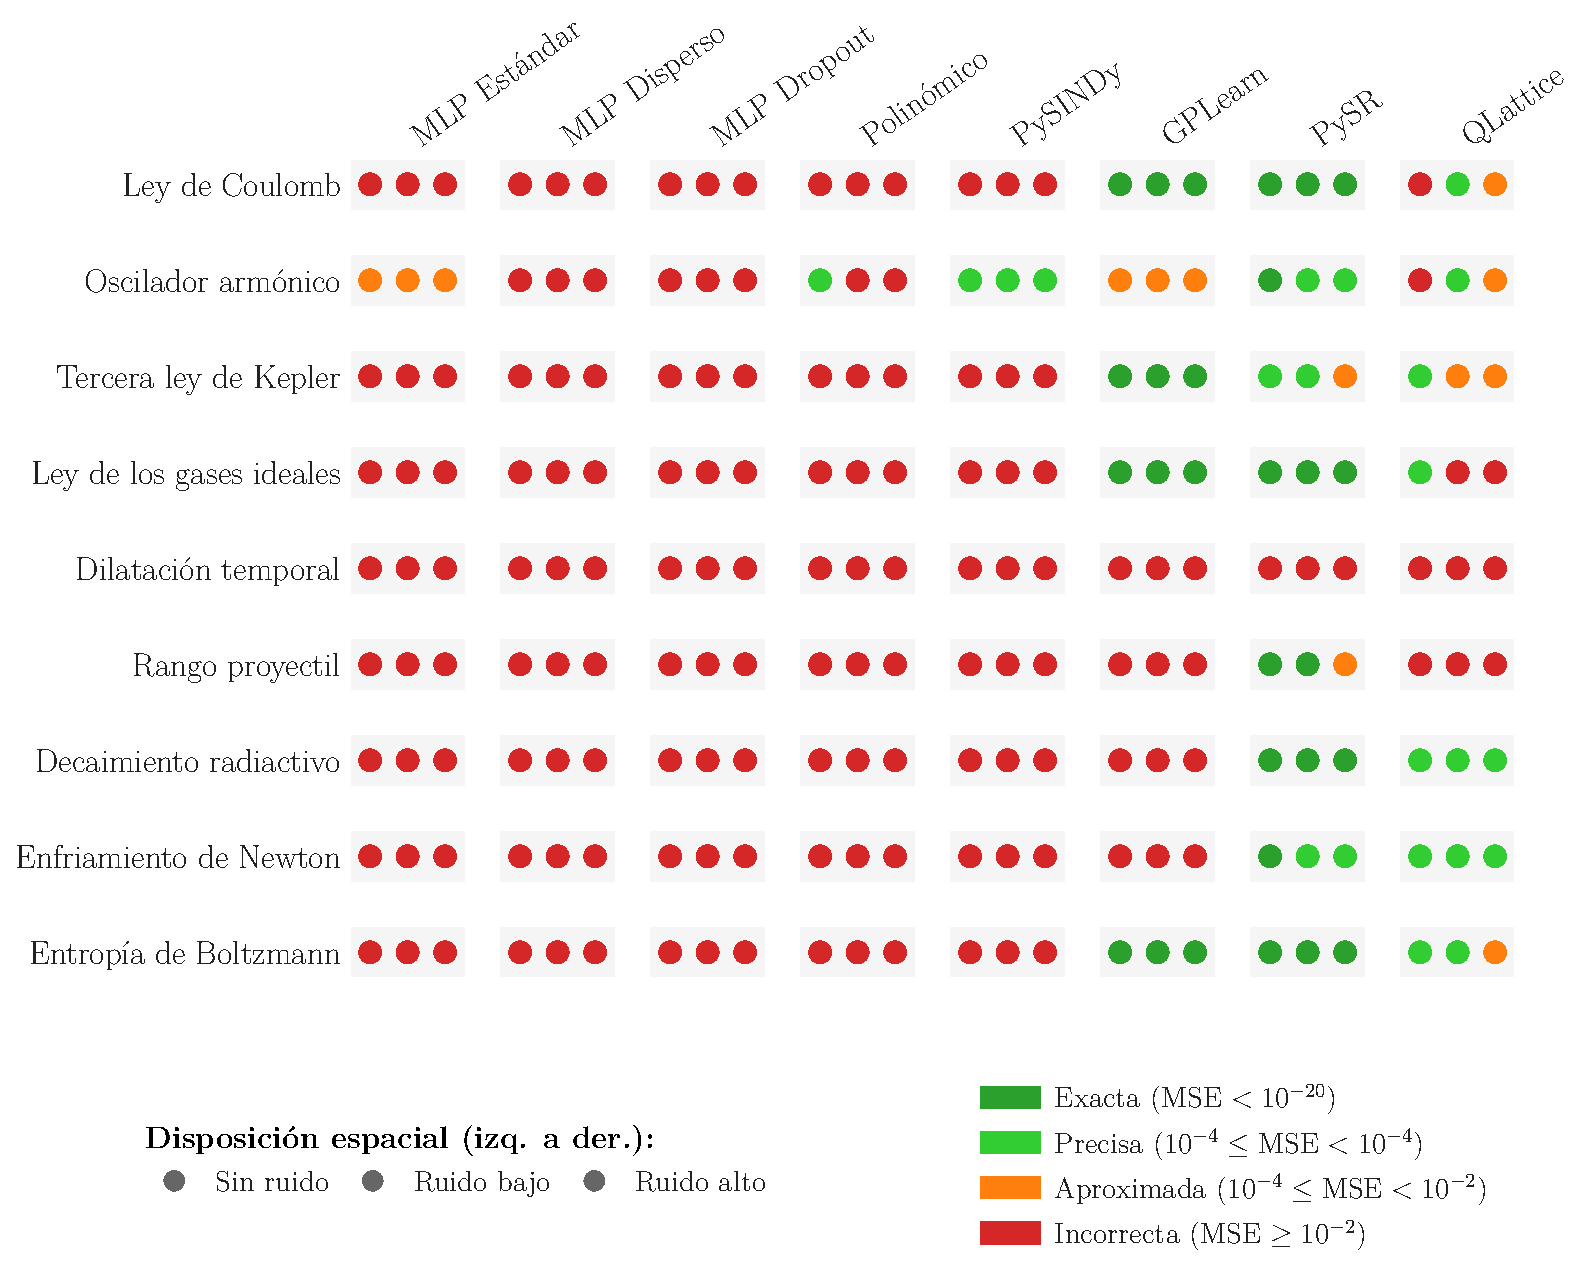
\includegraphics[width=\textwidth,height=0.8\textheight,keepaspectratio]{figures/model_recovery.pdf}
    \end{figure}
\end{frame}

% ─────────────────────────────────────────────────────────────────────────────

\begin{frame}{Análisis de Expresiones Recuperadas (Límite Determinista)}
    \begin{figure}
        \centering
        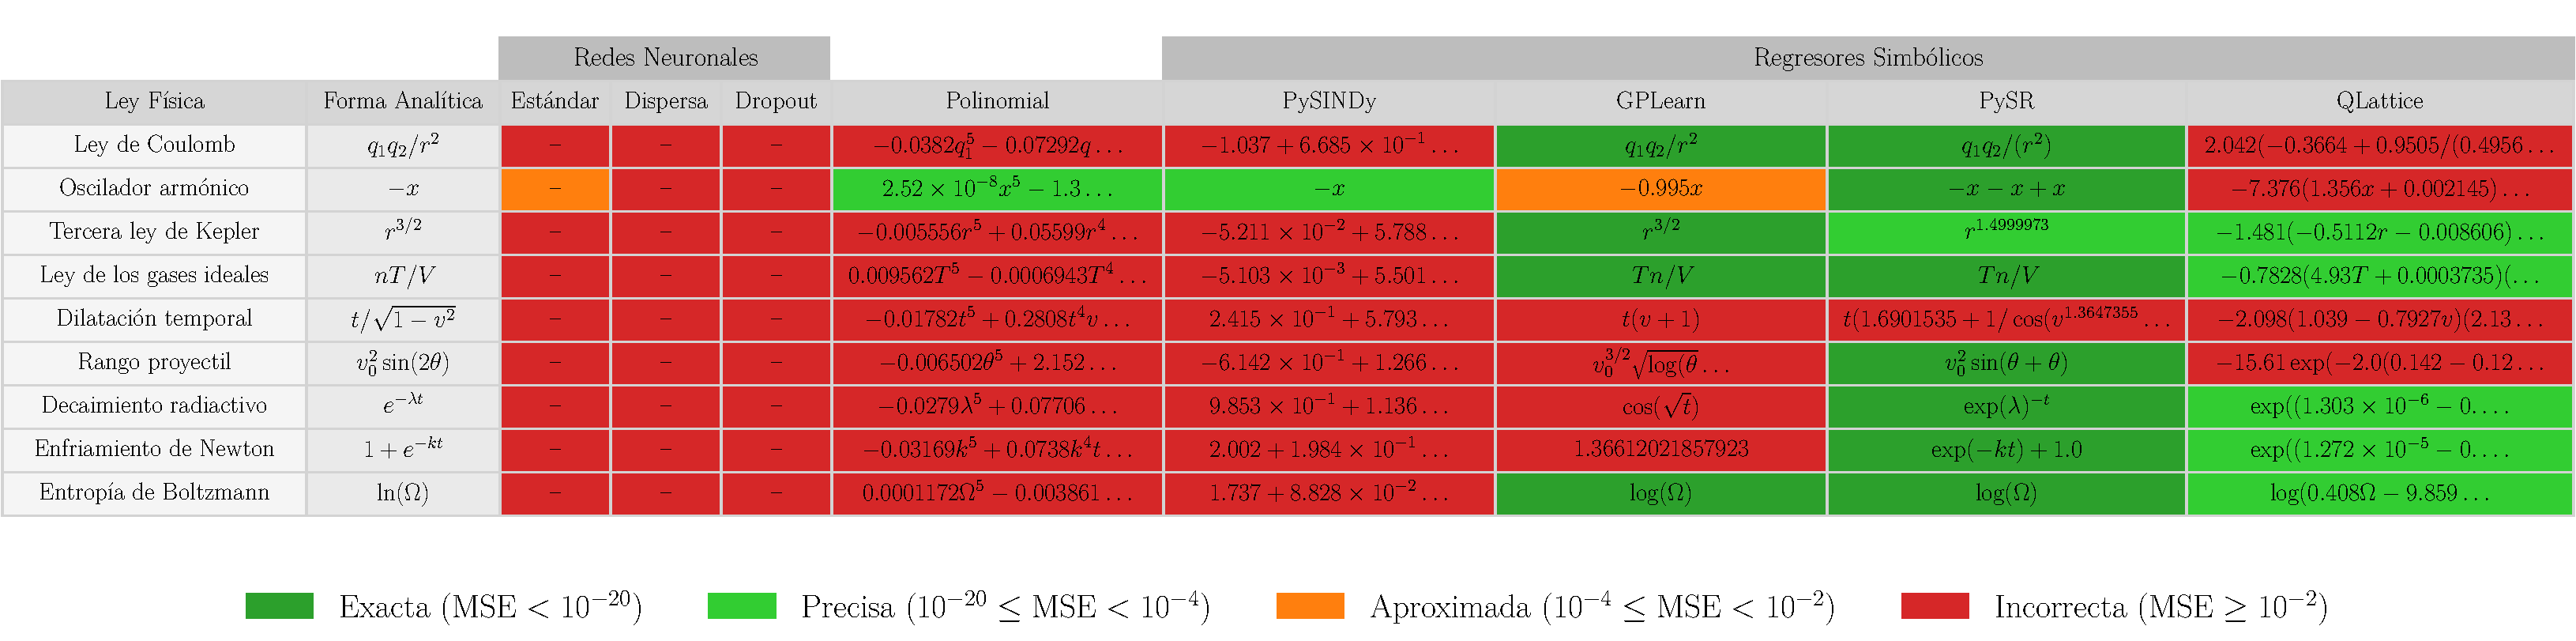
\includegraphics[width=\textwidth,height=0.8\textheight,keepaspectratio]{figures/table_no_noise.pdf}
    \end{figure}
\end{frame}

% ─────────────────────────────────────────────────────────────────────────────
\begin{frame}{Discusión Analítica}
    \begin{columns}[T]
        \column{0.48\textwidth}
        \textbf{Aproximadores Locales (MLP/Pol.)}
        \begin{itemize}
            \item Excelentes en el colector de datos de entrenamiento.
            \item Divergencia asintótica fuera de dominio (colapso OOD). 
            \item Carecen de invarianzas físicas intrínsecas o mecanismos para inferir la simetría de la ecuación.
        \end{itemize}

        \column{0.48\textwidth}
        \textbf{Regresores Simbólicos}
        \begin{itemize}
            \item Convergencia al límite analítico: MSE$_\text{OOD} \approx 0$ si se halla la topología subyacente.
            \item \textbf{PySR} exhibe robustez máxima frente a mínimos locales.
            \item \textbf{GPLearn} y \textbf{QLattice} penalizan fuertemente ante bases de operadores incompletas.
        \end{itemize}
    \end{columns}
    
    \vspace{0.6cm}
    \begin{block}{Impacto Estocástico (Ruido)}
        La adición de ruido $\varepsilon > 0$ introduce desviaciones en los tensores de constantes multiplicativas, pero \textbf{preserva la topología funcional} hallada por los algoritmos evolutivos en el 90\% de los casos.
    \end{block}
\end{frame}

% ─────────────────────────────────────────────────────────────────────────────
\begin{frame}{Conclusiones}
    \begin{block}{Jerarquía de Inferencia Asintótica}
        \centering\medskip
        \large \textbf{PySR} $\succ$ GPLearn $\approx$ QLattice $\succ$ PySINDy $\succ$ Polinomial $\gg$ Redes Neuronales
    \end{block}

    \vspace{0.5cm}
    \begin{enumerate}
        \item La inferencia de la estructura analítica formal es un requisito estricto para garantizar predictibilidad física fuera del dominio de entrenamiento.
        \item La parsimonia matemática actúa como el regularizador natural fundamental en el espacio funcional.
        \item Los algoritmos evolutivos (PySR) logran extraer la ley subyacente de los observables minimizando el sesgo teórico impuesto \textit{a priori}.
    \end{enumerate}


    
\end{frame}


\begin{frame}{Conclusiones}
    \begin{block}{Jerarquía de Inferencia Asintótica}
        \centering\medskip
        \large \textbf{PySR} $\succ$ GPLearn $\approx$ QLattice $\succ$ PySINDy $\succ$ Polinomial $\gg$ Redes Neuronales
    \end{block}

    \vspace{0.5cm}
    \begin{enumerate}
        \item La inferencia de la estructura analítica formal es un requisito estricto para garantizar predictibilidad física fuera del dominio de entrenamiento.
        \item La parsimonia matemática actúa como el regularizador natural fundamental en el espacio funcional.
        \item Los algoritmos evolutivos (PySR) logran extraer la ley subyacente de los observables minimizando el sesgo teórico impuesto \textit{a priori}.
    \end{enumerate}

    \vspace{5pt}
    \texttt{Código accesible en: \href{https://github.com/JorgeAcebes/symbolic-physics-discovery.git}{}https://github.com/JorgeAcebes/symbolic-physics-discovery.git}
\end{frame}


% ====================================================
%  DIAPOSITIVAS PREVENTIVAS (backup)
% ====================================================
\appendix
\section*{Apéndice: diapositivas de respaldo}

\begin{frame}{[Backup] ¿Por qué RandomSampler en lugar de TPE?}
  \begin{columns}[T]
    \begin{column}{0.55\textwidth}
      TPE (\textit{Tree-structured Parzen Estimator}) es el
      algoritmo por defecto de \texttt{Optuna}: modela la densidad
      de probabilidad de los hiperparámetros condicionada al historial
      de trials.\\[0.5em]
      \textbf{Problema en este contexto:}
      \begin{itemize}
        \item Espacio de hiperparámetros de alta dimensión
        \item Número reducido de iteraciones por presupuesto
              computacional
        \item TPE necesita muchas evaluaciones para construir
              un modelo de densidad fiable
      \end{itemize}
    \end{column}
    \begin{column}{0.42\textwidth}
      \begin{block}{RandomSampler como baseline}
        \begin{itemize}
          \item Muestreo uniforme $x_i \sim \mathcal{U}(\mathcal{X})$,
                independiente del historial
          \item Exploración insesgada
          \item Determinista: permite comparación reproducible
                entre modelos y leyes
          \item En régimen de pocos trials, comparable en rendimiento a TPE
        \end{itemize}
      \end{block}
    \end{column}
  \end{columns}
\end{frame}

\begin{frame}{[Backup] ¿Por qué GPLearn no recupera exponenciales?}
  \begin{columns}[T]
    \begin{column}{0.55\textwidth}
      El espacio funcional de GPLearn está definido por:
      \[
        \{+,\,-,\,\times,\,\div,\, \wedge,  \sin x,\,\cos x,\,x^{-1},\,\sqrt{x},\,\ln x\}
      \]
      \textbf{No incluye} $e^x$ ni composiciones que generen exponenciales.\\[0.5em]
      Para $N = e^{-\lambda t}$, GPLearn intenta aproximar
      la exponencial con sus operadores disponibles:
      \begin{itemize}
        \item $\cos(\sqrt{t})$ minimiza el MSE local dentro del rango
        \item Fuera del dominio, la aproximación diverge
        \item Resultado: MSE$_\text{OOD} \approx 0.29$, clasificado
              como \textbf{incorrecto}
      \end{itemize}
    \end{column}
    \begin{column}{0.42\textwidth}
      \begin{alertblock}{Sesgo del espacio funcional}
        Esta limitación no refleja una debilidad del algoritmo
        evolutivo en sí, sino una \textbf{decisión de diseño}
        sobre el diccionario de operadores.\\[0.4em]
        Incluyendo $e^x$ en el espacio funcional, GPLearn
        recuperaría las leyes exponenciales con la misma eficacia
        con que recupera las logarítmicas.
      \end{alertblock}
    \end{column}
  \end{columns}
\end{frame}

\begin{frame}{[Backup] ¿Por qué ningún modelo recupera la dilatación temporal?}
  \[
    t' = \frac{t}{\sqrt{1 - v^2}}
  \]
  \begin{columns}[T]
    \begin{column}{0.55\textwidth}
      \textbf{Problema de muestreo:}\\
      Con $v \sim \mathcal{U}(0, 1)$, la mayoría de puntos
      cae en la región $v \ll 1$ donde $t' \approx t$.
      La curvatura característica de la función solo se
      manifiesta para $v \to 1$, región sistemáticamente subrepresentada.\\[0.5em]
      \textbf{Consecuencia:}
      \begin{itemize}
        \item Los modelos aprenden $t' \approx t$ con pequeñas correcciones
        \item La topología funcional real (raíz cuadrada en denominador)
              no es detectada
        \item PySR aproxima: $t(v+1)$ o $t/\cos(v^{1.36})$
      \end{itemize}
    \end{column}
    \begin{column}{0.42\textwidth}
      \begin{block}{Solución propuesta}
        Un muestreo adaptativo con mayor densidad para $v \in [0.8, 1)$
        proveería la información necesaria para identificar la singularidad.
        \\[0.4em]
        Alternativamente, aumentar el número de épocas
        en PySR podría eventualmente encontrar la expresión exacta,
        a costa de mayor tiempo computacional.
      \end{block}
      \vspace{0.4em}
      \small
      \textbf{Conclusión:} limitación del \textit{protocolo experimental},
      no de los algoritmos.
    \end{column}
  \end{columns}
\end{frame}

\begin{frame}{[Backup] ¿Qué ventaja real ofrece PySR frente a GPLearn?}
  \begin{columns}[T]
    \begin{column}{0.50\textwidth}
      \textbf{Diferencias algorítmicas clave:}
      \begin{itemize}
        \item PySR usa \textbf{múltiples islas} (poblaciones paralelas)
              con migración por torneos $\to$ evita mínimos locales
        \item GPLearn usa una única población con presión
              de selección por torneo
        \item PySR construye un \textbf{frente de Pareto global}
              (complejidad vs.\ error) $\to$ selección óptima explícita
        \item PySR delega el cómputo pesado a \textbf{Julia}:
              mayor velocidad por generación
      \end{itemize}
    \end{column}
    \begin{column}{0.47\textwidth}
      \textbf{Espacio de operadores:}
      \begin{center}
        \small
        \begin{tabular}{lcc}
          \toprule
          Operador & GPLearn & PySR \\
          \midrule
          $+,-,\times,\div$ & \checkmark & \checkmark \\
          $\sin x, \cos x$ & \checkmark & \checkmark \\
          $\ln x, \sqrt{x}$ & \checkmark & \checkmark \\
          $e^x$ & \textbf{---} & \checkmark \\
          $x^a$ & \checkmark & \checkmark \\
          % $x \wedge y$ & --- & \checkmark \\
          \bottomrule
        \end{tabular}
      \end{center}
      \vspace{0.3em}
      \small
      El espacio más rico de PySR, combinado con la
      topología multi-isla, explica su ventaja en leyes
      con composiciones no triviales.
    \end{column}
  \end{columns}
\end{frame}

\begin{frame}{[Backup] PySR: Criterio de Selección de Modelos}
    \centering
    \textbf{Frontera de Pareto: Complejidad vs. Error}
    
    \vspace{0.3cm}
    \begin{tikzpicture}
        \begin{axis}[
            width=8cm, height=5.5cm,
            xlabel={\small Complejidad (Nodos del AST)},
            ylabel={\small Pérdida (MSE)},
            xmin=1, xmax=11, ymin=0, ymax=1,
            xtick={2, 4, 6, 8, 10},
            ytick={0, 0.5, 1.0},
            axis lines=left,
            grid=both,
            grid style={dashed, gray!30},
            clip=false
        ]
        
        % Observaciones subóptimas
        \addplot[only marks, mark=o, mark size=1.5pt, gray!60] coordinates {
            (3,0.85)(4.5,0.65)(5,0.70)(6.5,0.35)(7.5,0.18)
            (8,0.09)(9.5,0.042)(10,0.038)(2.5,0.80)(5.5,0.50)
            (7,0.22)(9,0.055)
        };
        
        % Frente de Pareto
        \addplot[uamblue, thick, mark=*, mark size=2pt] coordinates {
            (2,0.90)(3,0.72)(4,0.55)(5,0.38)(6,0.24)
            (7,0.13)(8,0.07)(9,0.04)(10,0.03)
        };
        
        % Punto óptimo elegido
        \addplot[only marks, mark=star, mark size=4pt, mark options={fill=exact, draw=exact}] coordinates {(7, 0.13)};
        
        \node[font=\footnotesize, right, text=exact] at (axis cs: 7.2, 0.18) {Selección Óptima};
        \end{axis}
    \end{tikzpicture}
    
    \vspace{0.2cm}
    La ecuación retornada es el vértice que maximiza la ganancia marginal de precisión por unidad de complejidad añadida.
\end{frame}

\section{Limitaciones}

\begin{frame}{[Backup] Limitaciones del estudio}
  \begin{enumerate}
    \item \textbf{Espacio de operadores heterogéneo entre modelos}\\
          GPLearn carece de operadores exponenciales; QLattice,
          de sinusoidales. Las diferencias de rendimiento reflejan
          decisiones de diseño, no solo la calidad del algoritmo.
    \vspace{0.4em}
    \item \textbf{Hiperparámetros promediados}\\
          Un único conjunto de hiperparámetros por modelo
          (media sobre \texttt{Optuna} por ley) es subóptimo
          para cada dataset particular; puede sesgar la comparativa.
    \vspace{0.4em}
    \item \textbf{Ausencia de análisis de varianza entre semillas}\\
          Los resultados son puntuales: sin intervalos de confianza
          no es posible afirmar significación estadística de las
          diferencias observadas.
    \vspace{0.4em}
    \item \textbf{Muestreo uniforme inadecuado para no linealidades locales}\\
          Leyes como la dilatación temporal tienen comportamiento relevante
          concentrado en una región. Un muestreo adaptativo mejoraría
          el condicionamiento del problema.
  \end{enumerate}
\end{frame}


\begin{frame}{[Backup] Curva de loss para MLP Estándar (Ley de Coulomb)}
    \begin{figure}
        \centering
        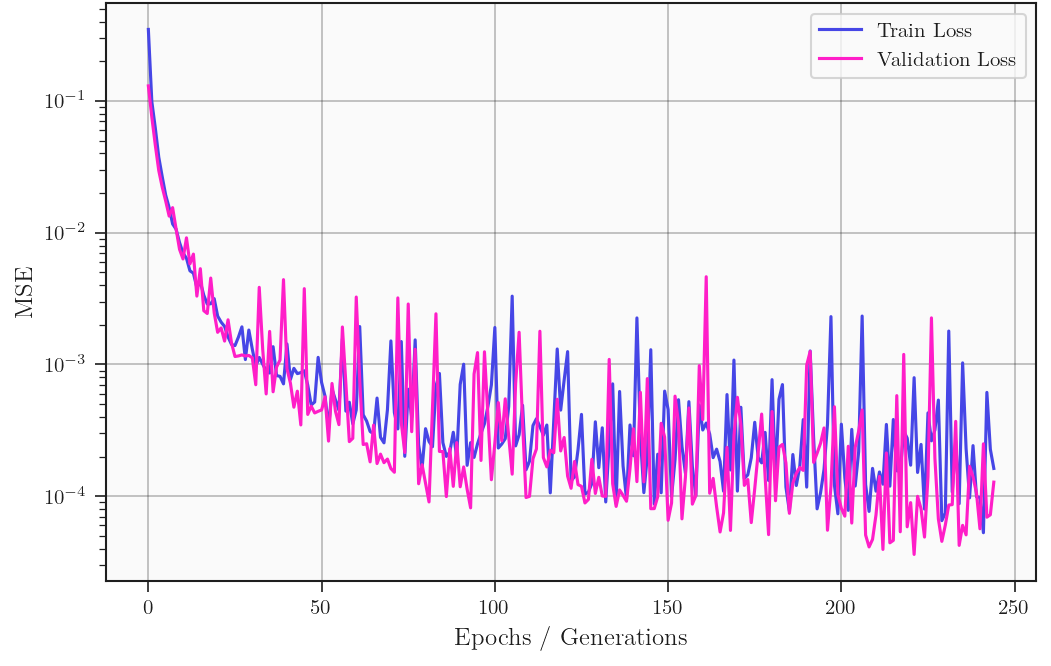
\includegraphics[width=\textwidth,height=0.8\textheight,keepaspectratio]{figures/coul_MLP.png}
    \end{figure}
\end{frame}

\begin{frame}{[Backup] Curva de loss para QLattice (Ley de Coulomb)}
    \begin{figure}
        \centering
        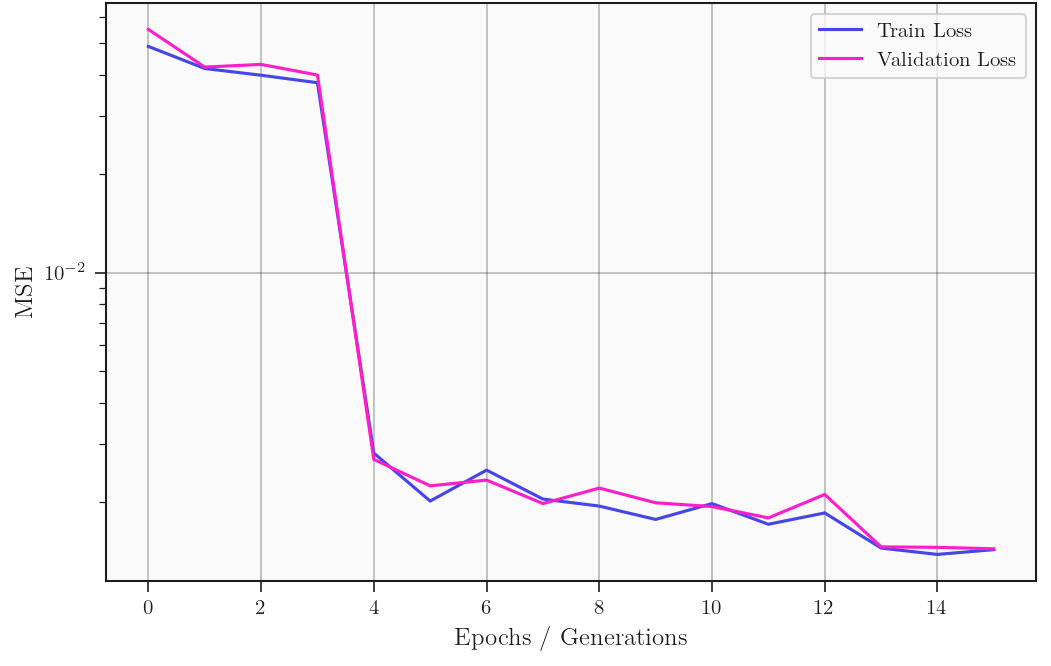
\includegraphics[width=\textwidth,height=0.8\textheight,keepaspectratio]{figures/coul_QLattice.png}
    \end{figure}
\end{frame}


\begin{frame}{[Backup] MSE OOD (Tercera Ley de Kepler)}
    \begin{figure}
        \centering
        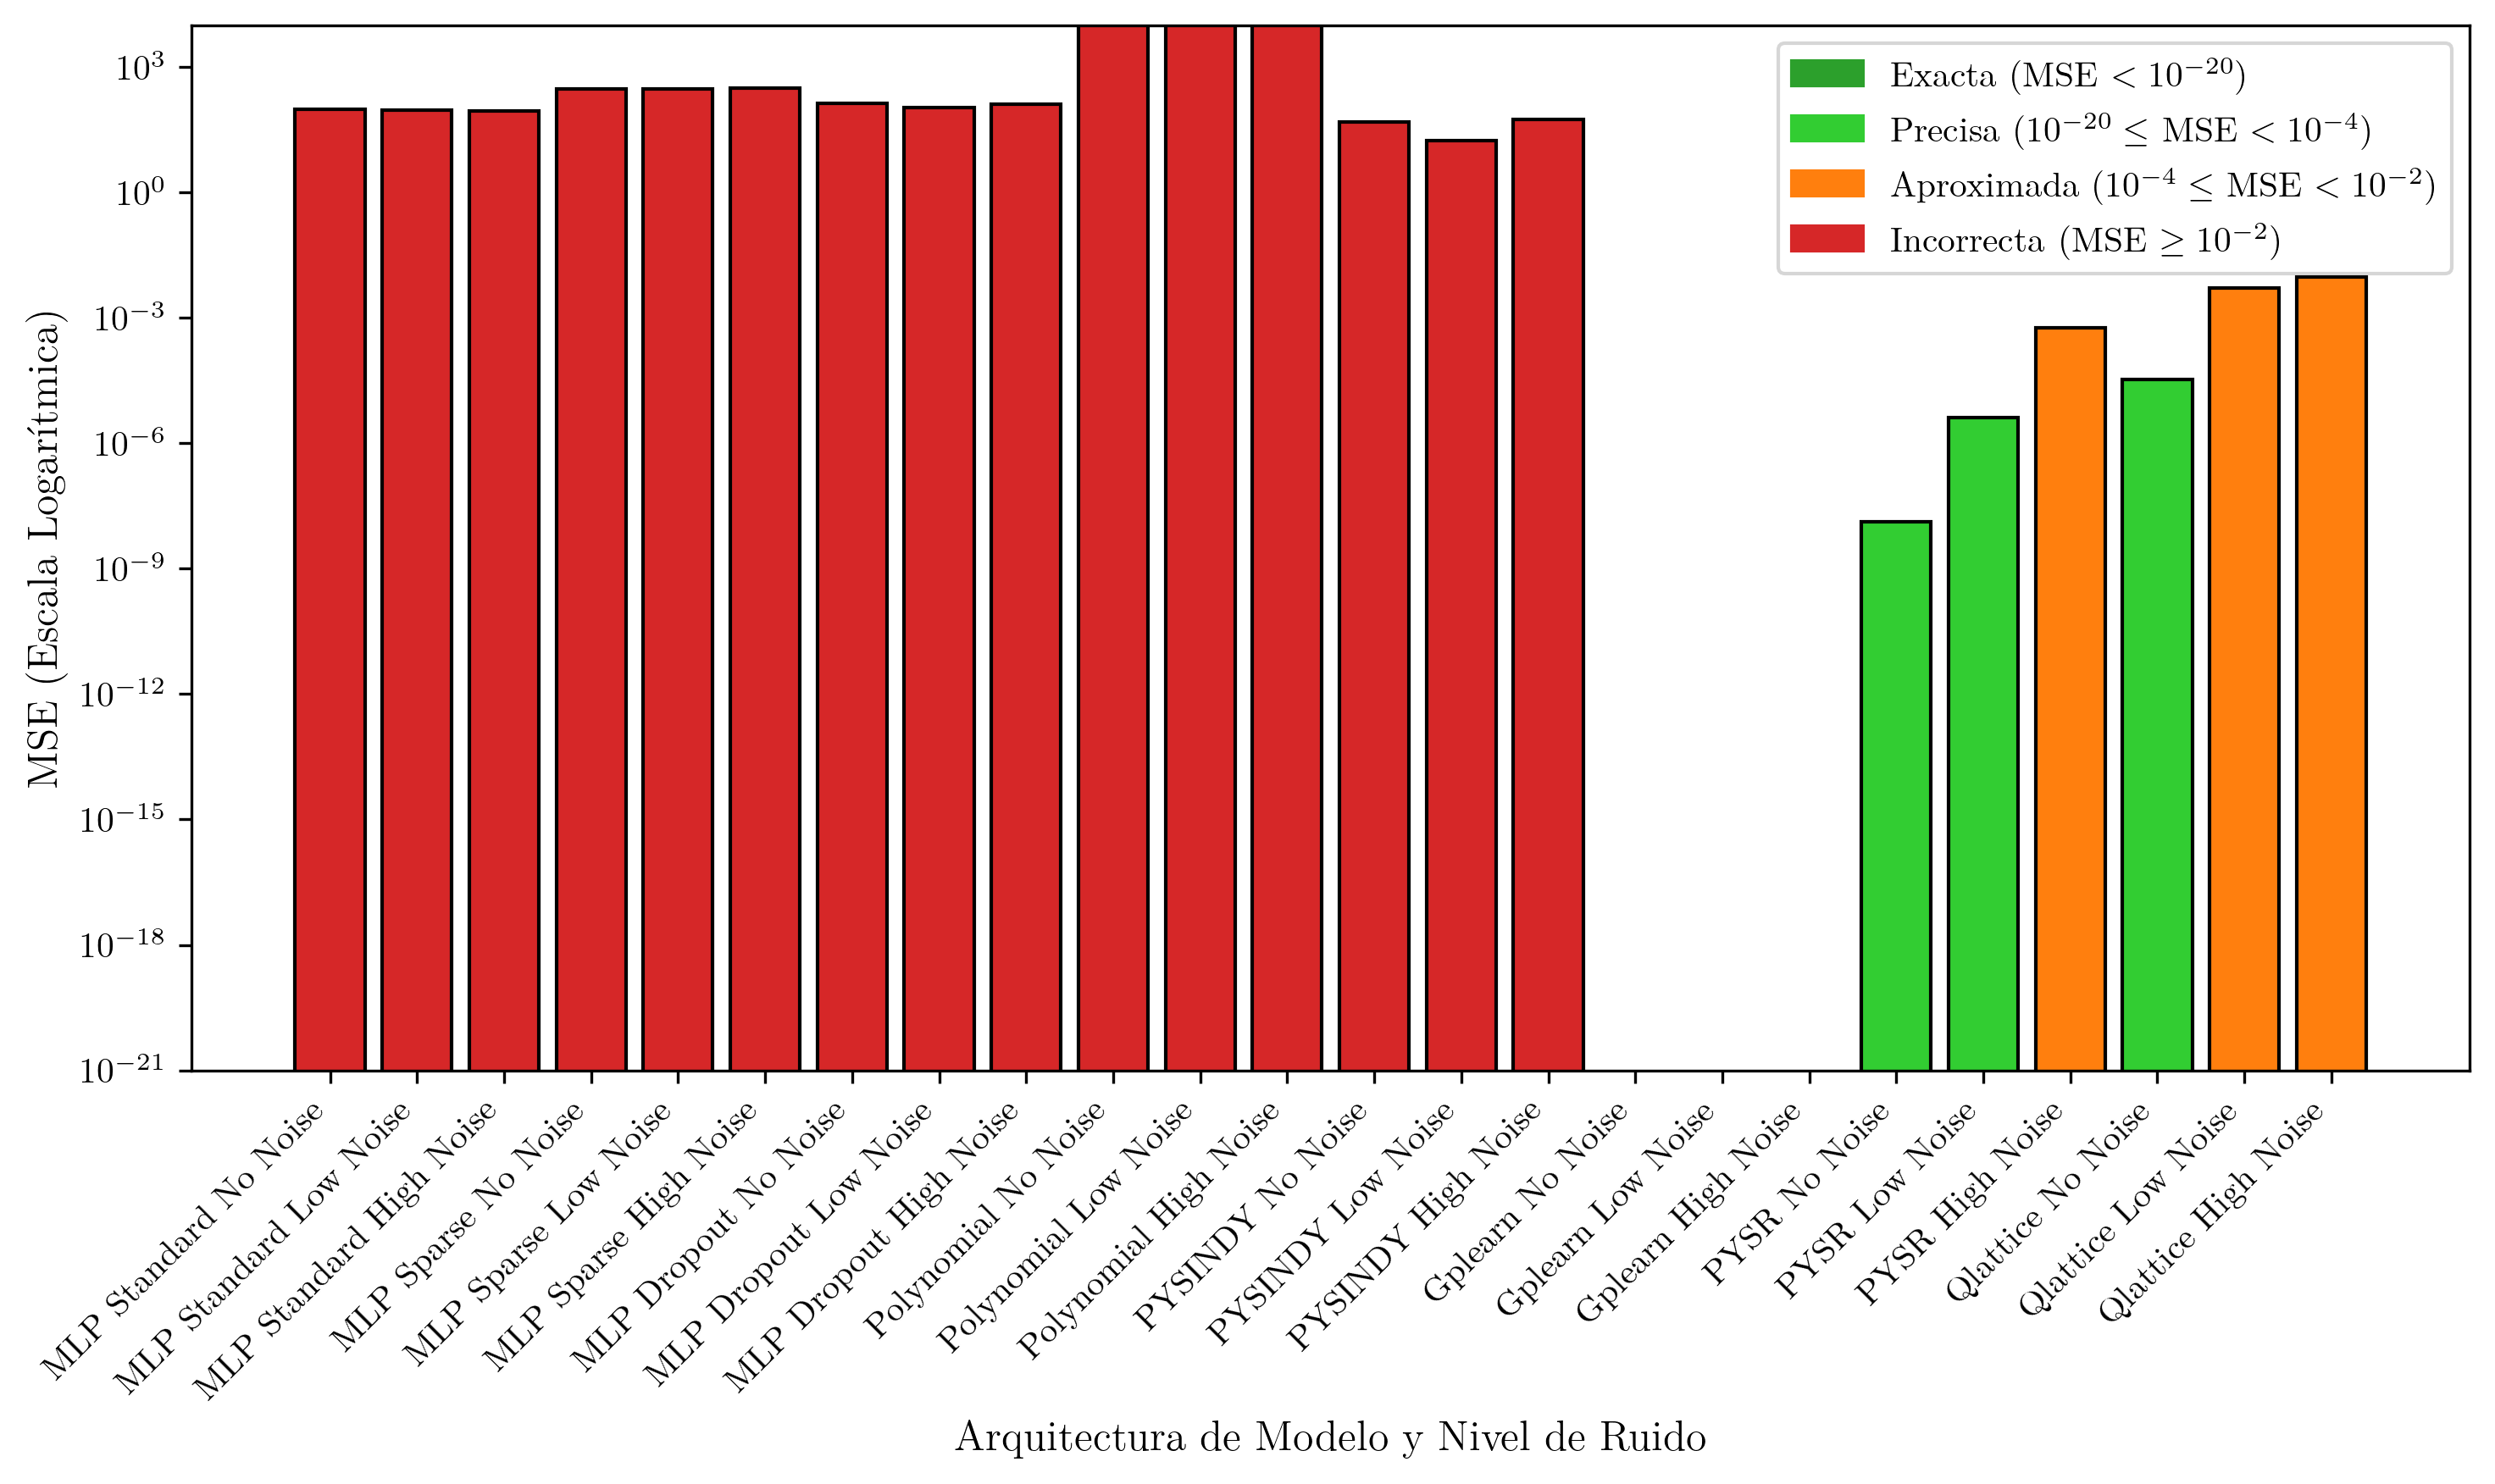
\includegraphics[width=\textwidth,height=0.8\textheight,keepaspectratio]{figures/kepler_mse_ood.png}
    \end{figure}
\end{frame}


\begin{frame}{[Backup] MSE OOD (Oscilador Armónico)}
    \begin{figure}
        \centering
        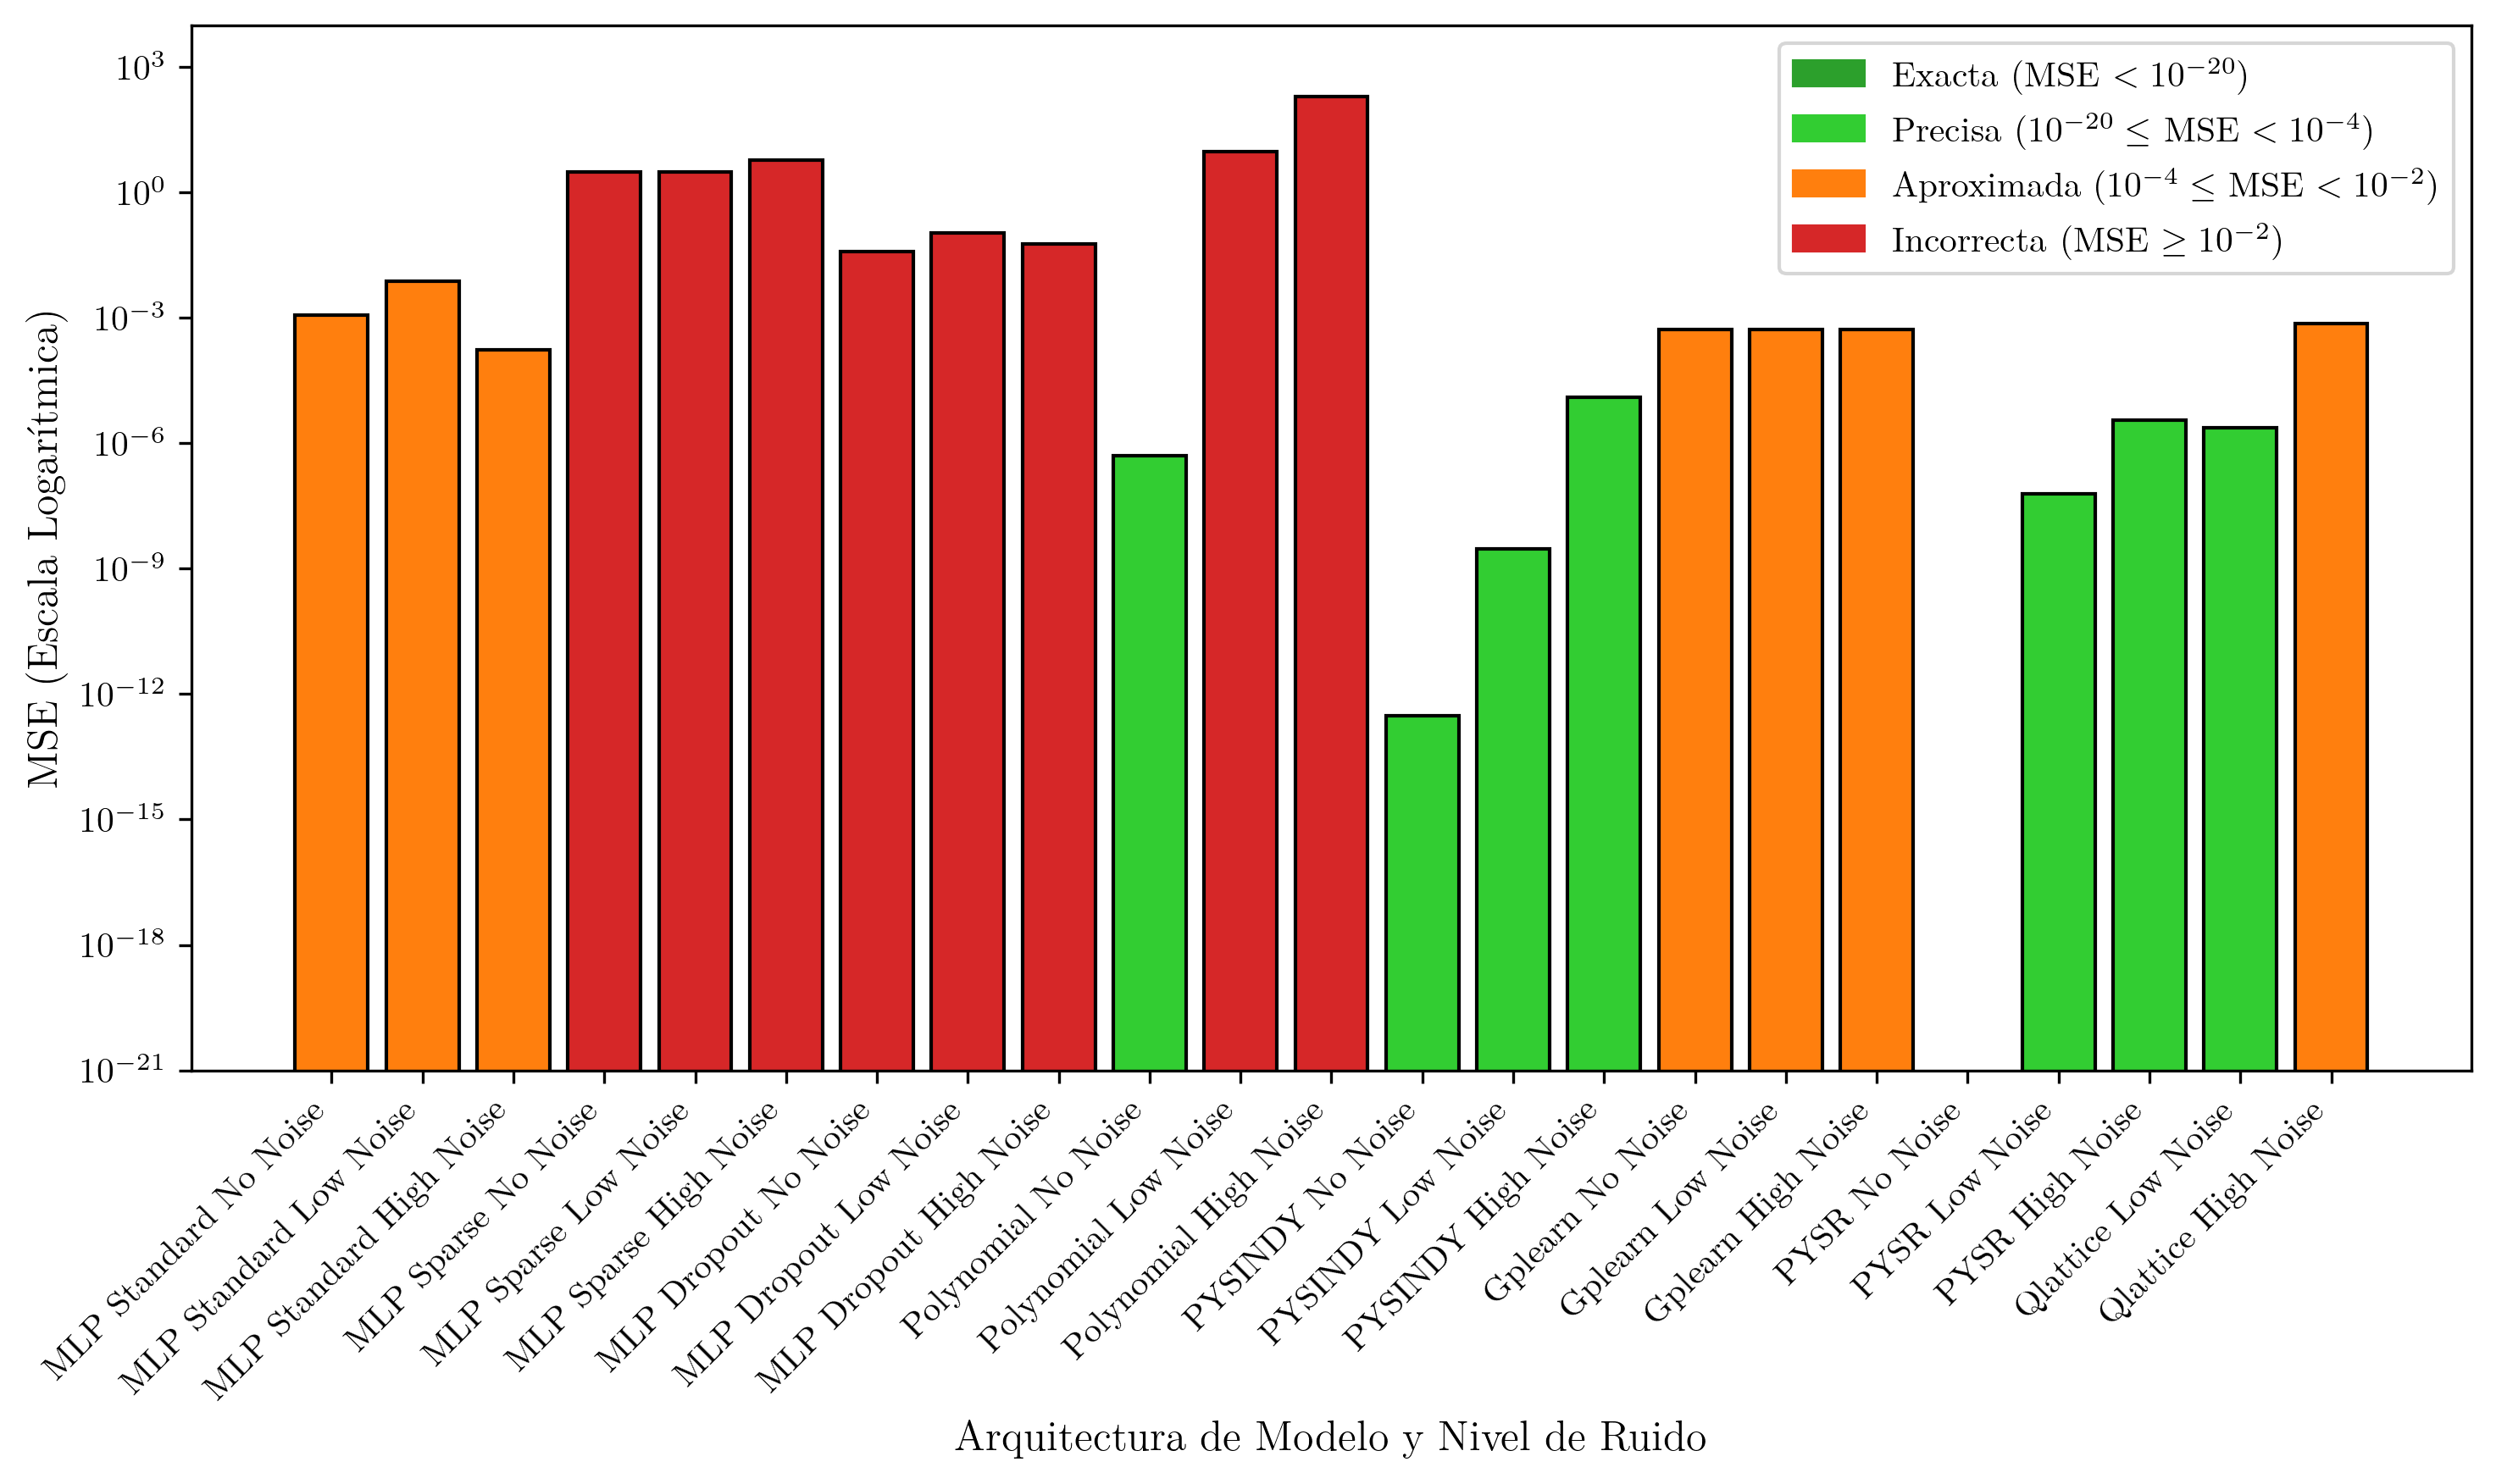
\includegraphics[width=\textwidth,height=0.8\textheight,keepaspectratio]{figures/oscillator_mse_ood.png}
    \end{figure}
\end{frame}


\begin{frame}{[Backup] Análisis de Expresiones Recuperadas (Ruido Bajo)}
    \begin{figure}
        \centering
        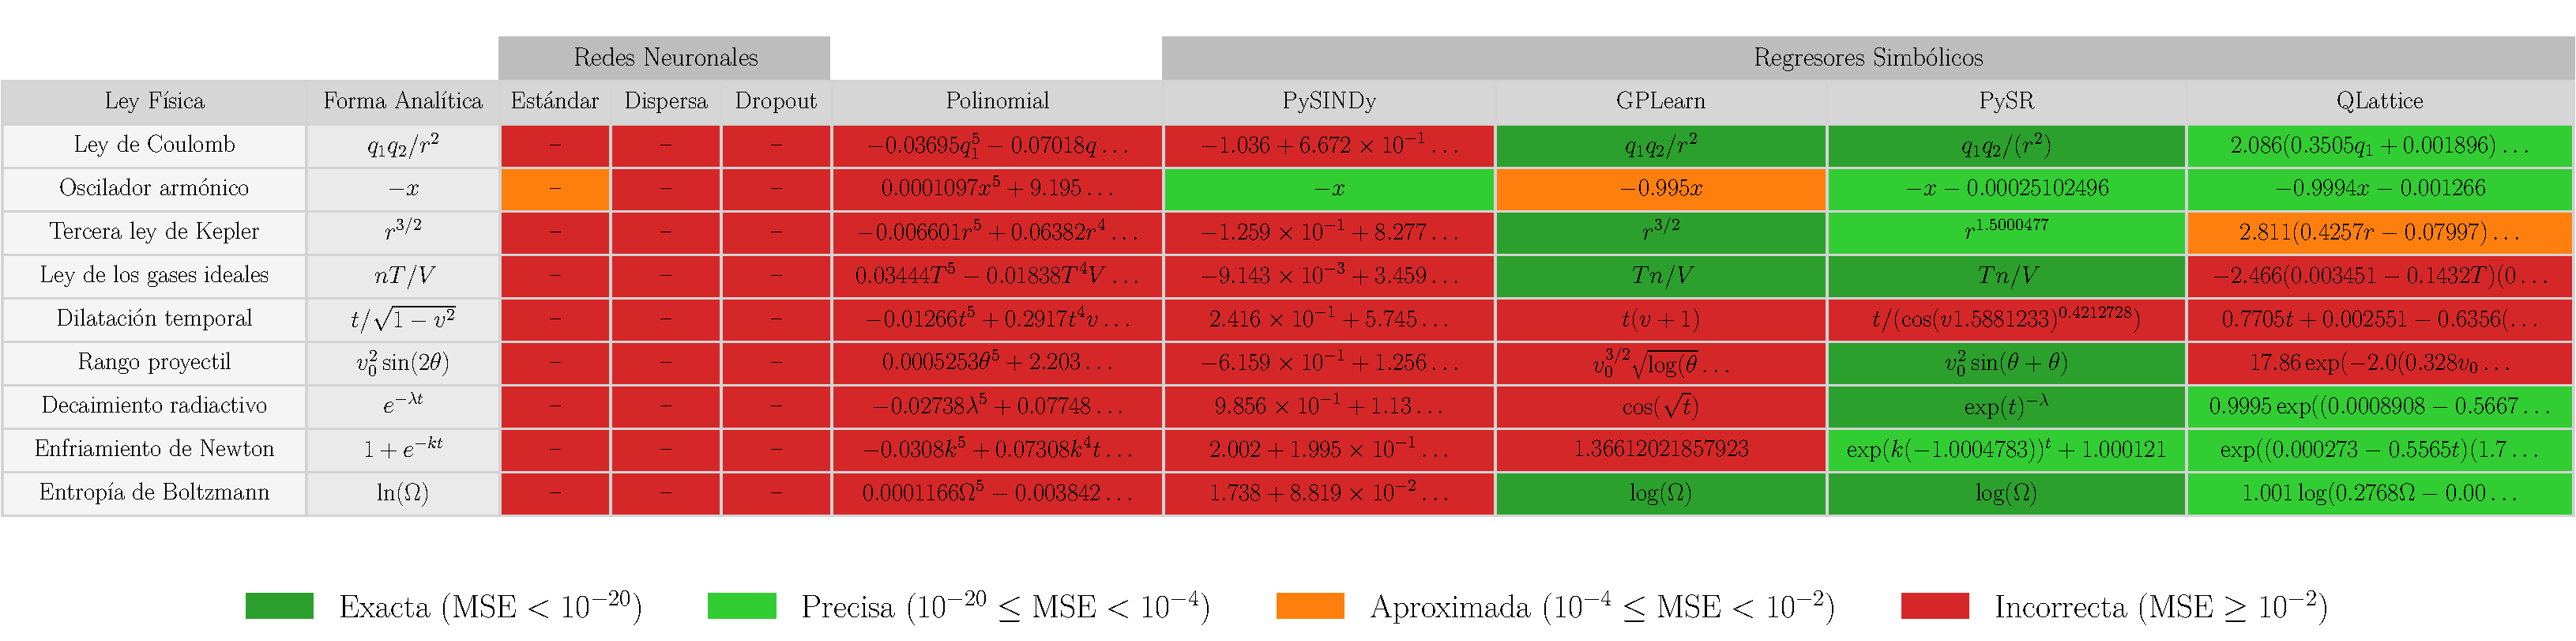
\includegraphics[width=\textwidth,height=0.8\textheight,keepaspectratio]{figures/table_low_noise.pdf}
    \end{figure}
\end{frame}

\begin{frame}{[Backup] Análisis de Expresiones Recuperadas (Ruido Alto)}
    \begin{figure}
        \centering
        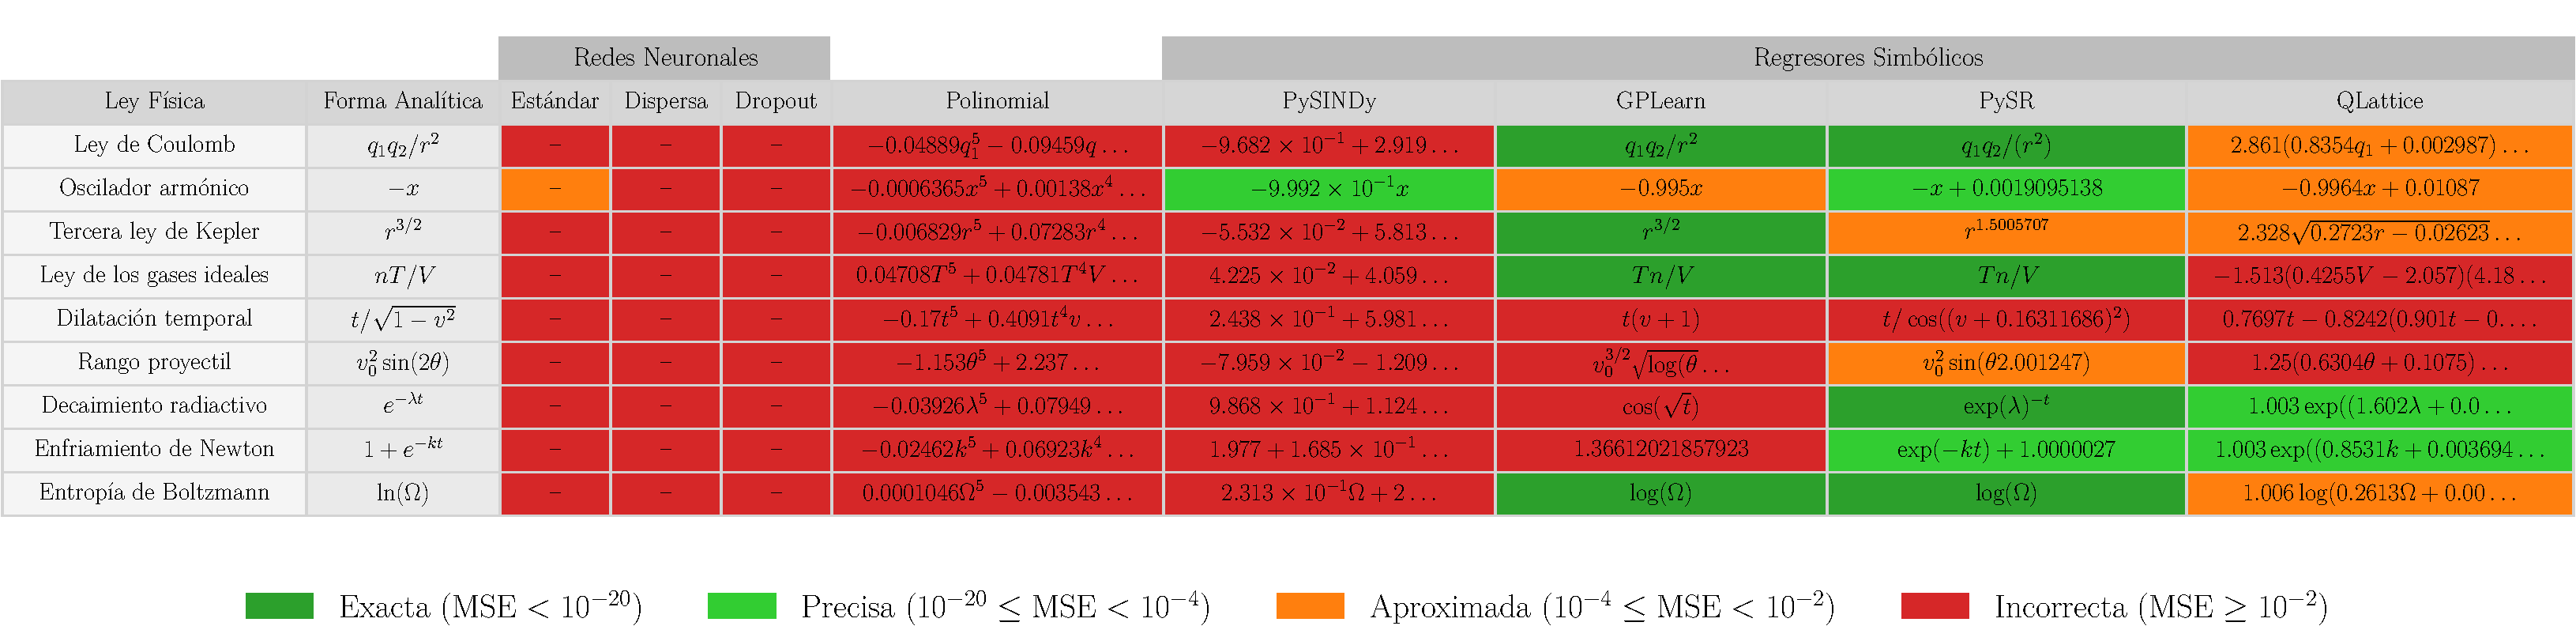
\includegraphics[width=\textwidth,height=0.8\textheight,keepaspectratio]{figures/table_high_noise.pdf}
    \end{figure}
\end{frame}

% =============================================================================
\end{document}

